\chapter{Diseño de la solución}
\label{chap:diseño}

\section{Arquitectura del sistema propuesto}

El sistema propuesto está orientado a ser distribuido y escalable. Además, permite que cualquier aplicación use si esquema de 
autenticación. 
El echo de que use un servidor de autenticación centralizado simplifica la gestión de reglas de acceso y reduce complejidad en 
la revocación de certificados.

En la figura \ref{fig:multauth-diseño} se muestra cómo es la interconexión entre los distintos elementos. A este diseño hay que
añadir dos elementos adicionales: el broker MQTT y el servidor de configuración, tal y como se muestra en \ref{fig:mqtt-topology}.

\begin{figure}[H]
    \centering
    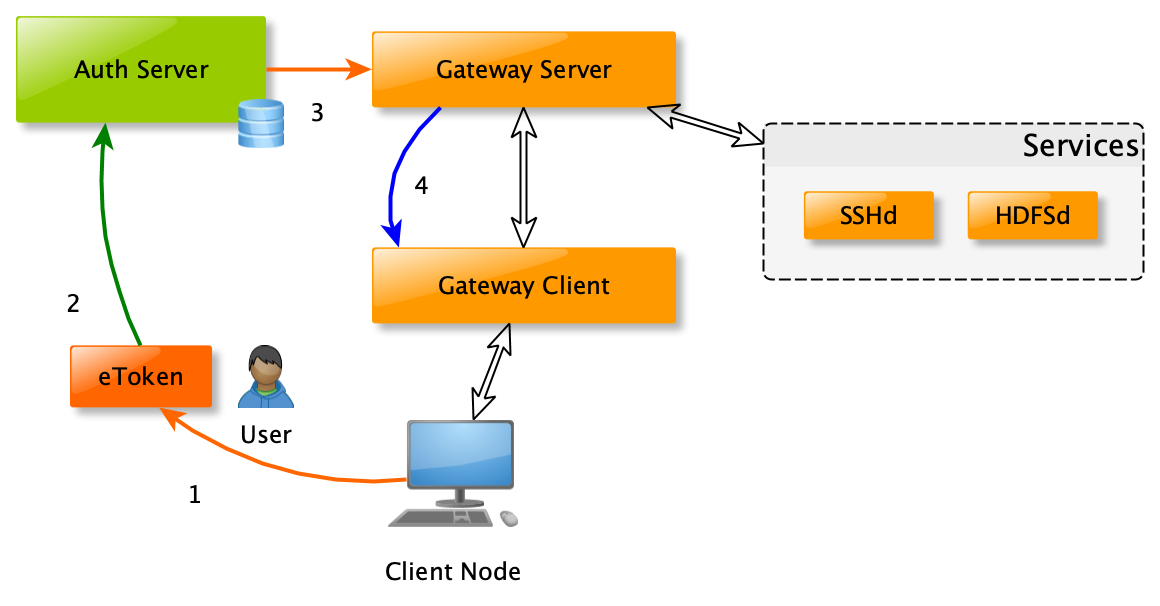
\includegraphics[scale=0.25]{global_topology_v1.png}
    \caption{Diseño del sistema propuesto en \cite{multipauthpaper}}
    \label{fig:multauth-diseño}
\end{figure}

\begin{figure}[H]
    \centering
    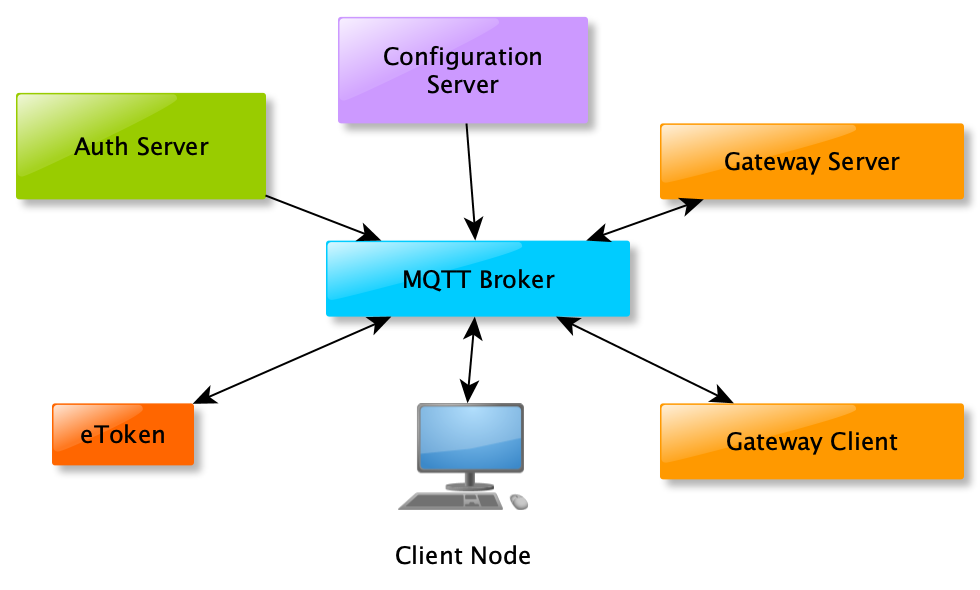
\includegraphics[scale=0.25]{global_topology_mqtt_v1.png}
    \caption{Topología MQTT}
    \label{fig:mqtt-topology}
\end{figure}

\section{Fases de la solución}

La solución propuesta en la sección\ref{sec:motivacion} se ha desarrollado siguiendo las siguientes fases: una primera etapa de preparación de
entorno seguro, una segunda etapa de identificación, y una final de autenticación. Para cada una de las fases se adjunta una 
diagrama de secuencias \footnote{Los valores entre $<$ y $>$ indican un valor en concreto, no el valor definido entre ambos 
símbolos} \footnote{Los tópicos tienen la estructura emisor/receptor/item}

\subsection{Fase TLS}
\label{sec:tls_phase}

En esta fase, el broker MQTT debe crear un certificado firmado por una CA para verificar su identidad. 
Para comunicarse por TLS con el broker MQTT, se ha llevado a cabo los siguientes pasos:

\begin{enumerate}
    \item Crear la clave privada de la CA
    \item Crer el certificado CA usando la clave privada del paso 1 para firmarla
    \item Crear la clave privada del broker MQTT
    \item Crear la solicitud de firma de certificados (\acf[first-style=short]{csr}) para el broker MQTT usando la clave privada del paso 3
    \item Usar la clave y certificado CA para firmar el certificado del broker MQTT
    \item Enviar el certificado del paso 5 al broker MQTT
    \item Distribuir el certificado CA a los cliente que se quieran comunicar a través del broker MQTT 
\end{enumerate}

\begin{figure}[H]
    \centering
    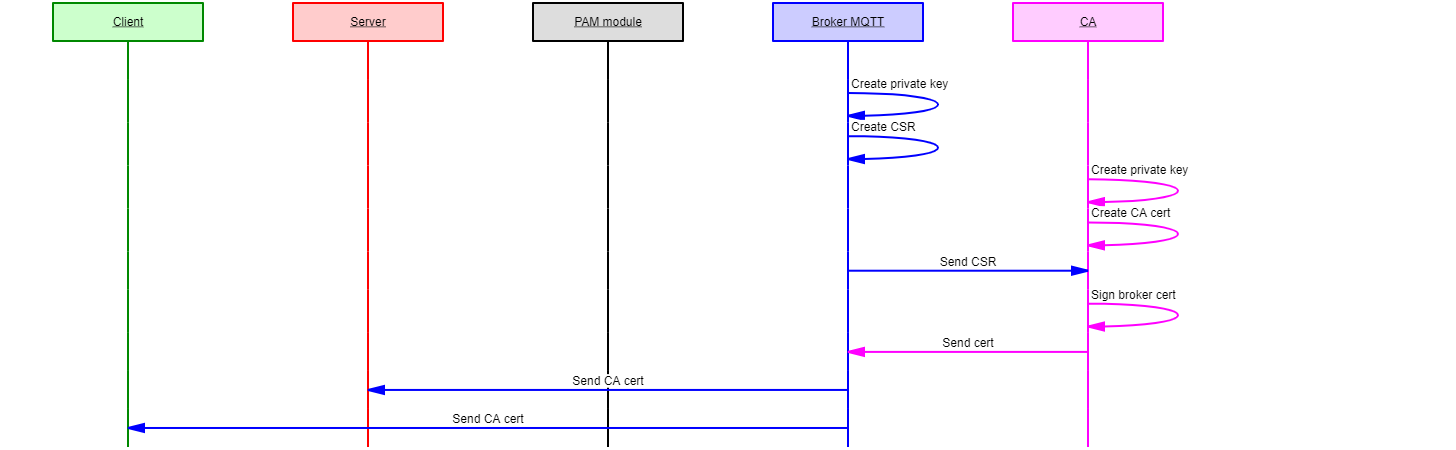
\includegraphics[scale=0.25]{tls_phase.png}
    \caption{Fase TLS}
\end{figure}

Como último paso, el archivo de configuración del cliente \textit{mosquitto} en el broker MQTT tiene que indicar la clave y 
certificados necesarios tal y como figura en \ref{code:pam_conf}.

Si un cliente quiere usar el broker MQTT para publicar un mensaje o subscribrse a un tópico, necesita ``mostrar'' el certificado
CA al broker MQTT. No es la única forma de identificación vía TLS. También existe la opción de que cada cliente
cree su propio certificado firmados por la CA.

\subsection{Fase de identificación}
\label{sec:id_phase}

En esta fase, el cliente se tiene que registrar en el servidor para poder usar su servicio. Para ello, el cliente crea un 
identificador único \acf[first-style=short]{uuid} y un par de claves pública y privada. Estos se guardan en un directorio en concreto. Se ha
escogido \textit{.anubis} en la carpeta \textit{home} del usuario. Las claves se guardan con el UUID como nombre del archivo 
($<uuid>.pem y <uuid>.key$) y finalmente se envía la clave pública al servidor. Se puede usar el protocolo \acf[first-style=short]{scp}. Dado que 
no se quiere usar un método de autenticación distinto al propuesto por este trabajo, se podría crear una clave pública temporal del 
servidor y subirla a algún servidor de claves públicas. El cliente por tanto podría usarla para mandar su clave pública a su 
directorio \textit{.anubis} de forma segura y una vez envíada, eliminarla. Una vez que el servidor tiene la clave pública del 
cliente, este lo registra en el archivo de configuración de usuario \ref{code:user_conf}. Este indica el UUID concreto para un 
usuario en el sistema. Se usa en caso de que el usuario tenga varias claves públicas y por tanto el servidor sepa que clave usar 
para la autenticación.

\begin{figure}[H]
    \centering
    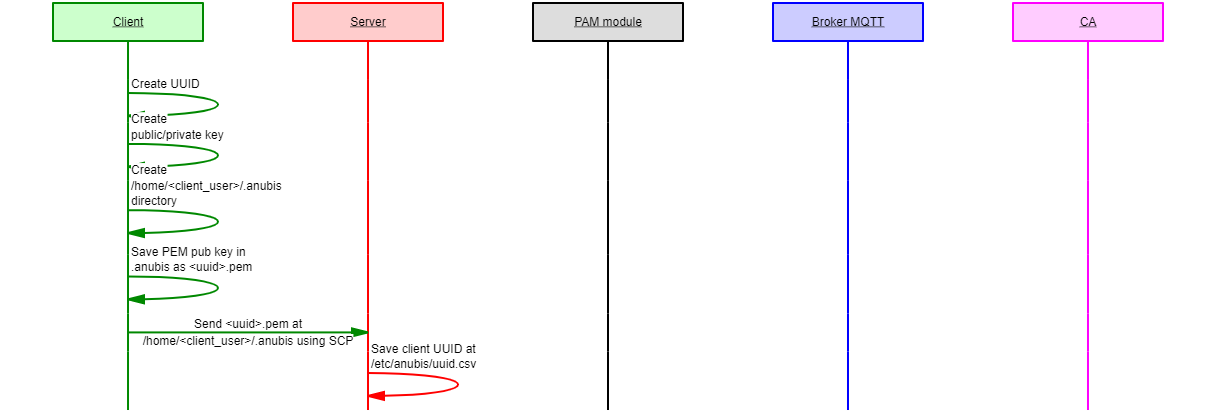
\includegraphics[scale=0.25]{id_phase.png}
    \caption{Fase de identificación}
\end{figure}

\subsection{Fase de autenticación}

En esta fase reside el proces de autenticación del cliente contra el servidor una vez que se ha establecido un canal seguro y 
registrado el cliente en el mismo.

El cliente se subscribe al tópico $pam/<uuid>/challenge$ por el cual recibirá el desafío y envía una petición para 
abrir una sesión por SSH al servidor. 

Al llegar la petición SSH al servidor, este comprueba que almacena el nombre del usuario que se quiere autenticar y comprueba su UUID 
en el archivo de configuración de usuarios \ref{code:user_conf} ($/etc/anubis/uuid.csv$). Este es un archivo de valores separados
por coma (CSV), el usuario y su UUID asignado. Una vez el servidor conoce el UUID, de plantean dos posibilidades:

\begin{enumerate}
    \item Que el usuario no necesite autenticarse de la forma propuesta
    \item Que el usuario tenga que autenticarse
\end{enumerate}

Cada condición se da según la política definida en el archivo de configuración de anubis \ref{code:anubis_conf}. Existen dos 
tipos de políticas:

\begin{enumerate}
    \item \textit{relax}: no es necesario aplicar la autenticación
    \item \textit{strict}: se aplica la autenticación
\end{enumerate}

La política \textit{relax} es útil en casos en los que por ejemplo el usuario provenga de una red de confianza como puede ser una
Universidad. En ese caso, el módulo PAM propuesto devolvería un $PAM_IGNORE$ pasando el siguiente módulo. En caso de la 
política \textit{strict}, es necesario ejecutar el proceso de autenticación propuesto y que devuelva un $PAM_SUCCESS$.

Una vez que se compruebe el UUID del usuario, si la política es de tipo \textit{strict}, el servidor se subscribe a dos tópicos:

\begin{itemize}
    \item $<uuid>/pam/r$
    \item $<uuid>/pam/s$
\end{itemize}

Por esos tópicos, el cliente publicará el par de valores [$r, s$] del algoritmo ECDSA definido en \ref{subsec:ecdsa} en formato 
hexadecimal.

Seguidamente, crea el desafío y lo publica al tópico $pam/<uuid>/challenge$. El desafio es una cadena de 64 caracteres aleatoria
compuesta de números y letras. Al llegar el mensaje al broker MQTT, este lo reenvía a todos los nodos que estén suscritos a dicho 
tópico. Dado que solo hay un UUID por cliente, el mensaje solo le llega al cliente determinado por el UUID. 

El cliente crea el hash del desafío usando el algoritmo SHA-512 dado su robustez con respecto a otros de menor tamaño como puede 
ser SHA-256. Una vez que tiene el hash, lo firma usando su clave privada creada en \ref{sec:id_phase} y envía ambos valores $[r,s]$ 
por los tópicos $<uuid>/pam/r$ y $uuid>/pam/s$ respectivamente siendo estos retransmitidos por el broker MQTT al servidor.

El servidor recibe ambos valores [$r, s$] para crear la firma de curva elíptica y crea el hash del desafío. A continuación verifica
el hash usando la firma generada anteriormente y la clave pública de tal forma que:

\begin{itemize}
    \item Si el cliente es quien dice ser, la verificación es correcta ya que solo el cliente verídico tiene la clave privada
    \item Si el desafío ha sufrido alguna modificación por la intervención de una tercera persona, la verificación saldrá incorrecta
\end{itemize}

Una verificación correcta devuelve $PAM_SUCCESS$ mientras que una errónea devuelve $PAM_AUTH_ERR$, siendo estas variables globales
de la librería de PAM.  

\begin{figure}[H]
    \centering
    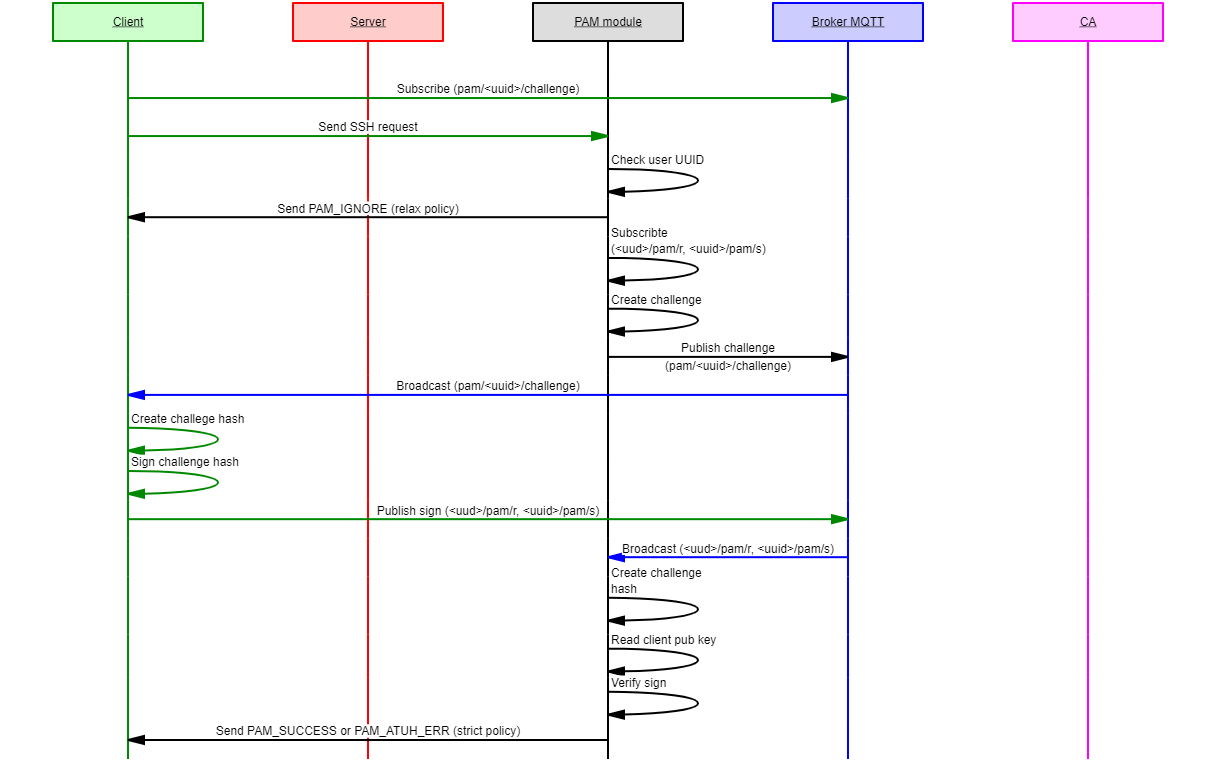
\includegraphics[scale=0.25]{auth_phase.png}
    \caption{Fase de autenticación}
\end{figure}

En la siguiente imagen se mustra la topología global del sistema propuesto:

\begin{figure}[H]
    \centering
    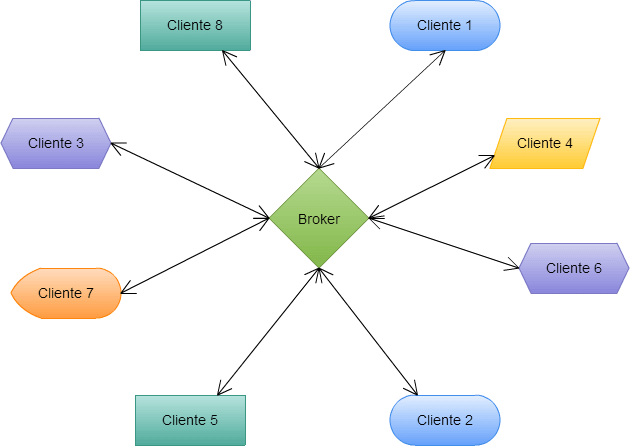
\includegraphics[scale=0.15]{topologia.png}
    \caption{Topología del diseño}
\end{figure}

\section{Código fuente}

El código fuente no se adjunta por simplicidad y limpieza en la memoria pero se encuentra subido a la plataforma de GitHub 
\cite{garcia_sergiogp98mqtt-pam_2021}. 

\section{Entorno de virtualización}

Tal y como se ha mencionado en \ref{sec:analisis-herramientas}, en vez de usar un ESP-32 como eToken de autenticación y un servidor 
físico que recrearía un escenario real, he decido virtualizar el entorno usando máquinas virtuales gracias al programa 
\textit{open-source} de Oracle \textit{Vagrant}.

\textit{Vagrant} es una herramienta destinada a la creación y configuración de entornos de desarrollo. Orginariamente fue 
desarrollado para que trabajase con entornos que corriesen bajo el hipervisor de \textit{VirtualBox} \cite{virtualbox}, siendo 
este un software de virtualización desarrollado por la propia Oracle.

Actualmente, $Vagrant$ funciona con otros hpervisores como el de Windows $Hyper-V$, el famoso $VMware$ así como entornos en la 
nube tales como $DigitalOcean$ o $Amazon Web Services$. Está desarrollado en Ruby pero se puede usar en proyectos de diversos 
lenguajes de programación.

Gracias a su facilidad de despliegue y rapidez a la hora de escalar, me ha permitido crear entornos complejos para probar el 
sistema propuesto.

$Vagrant$ require de un archivo de tipo \acf[first-style=short]{yaml} para su configuración que se llama $Vagrantfile$. Para este 
proyecto se ha escrito el siguiente archivo de configuración \ref{code:vagrantfile} compuesto de dos parte:

\begin{enumerate}
    \item El método $add_ssh_key$ añade la clave pública a la máquina virtual creada
    \item La parte de configuración de las máquinas virtuales: broker MQTT, cliente y servidor
\end{enumerate}
